% APA style article template

\documentclass[a4paper,man,floatsintext,12pt]{apa6} % 'man' gives you a one column manuscript layout, floatsintext forces the images to appear in the text, rather than the end of the manuscript (remove this if you want the images at the end)
%\documentclass[a4paper,jou,12pt]{apa6} % 'jou' gives you a two column journal layout. 12pt is the font size.

\usepackage[utf8]{inputenc}
\usepackage{graphicx}
\usepackage[left]{lineno}
\usepackage[english]{babel}
\usepackage[round]{natbib} % referencing style
\bibliographystyle{newapa} % APA referencing style
\usepackage[colorlinks, citecolor = black, urlcolor = black]{hyperref} % allows you to put in a URL to your data
\graphicspath{ {Images/} } % Images should be put into the folder 'Images'

%\thispagestyle{otherpage} % this line removes the running head if you don't want it

\title{Title} 
\shorttitle{Running head} % leave this empty if you don't want a running head
\author{Authors}
\affiliation{Affiliation}


\abstract{Enter abstract text here}
\keywords{Enter keywords here}
\authornote{Correspondence regarding this article should be addressed to XXX at XXX (email: XX).}


\begin{document}

\maketitle
\linenumbers % remove this to remove line numbers


\section{Introduction}

Type the introduction here...

\section{Materials and methods} % the sections included will vary based on your paper

\subsection{Participants}

Type the participant information here...

\subsection{Stimuli and Presentation}
\subsection{Analysis}

\section{Results}


% Inset a figure
\begin{figure}[h!] % man puts the images at the end of the text, unless you include floatsintext in the \manuscript line at the top of this page.
	\centering	
	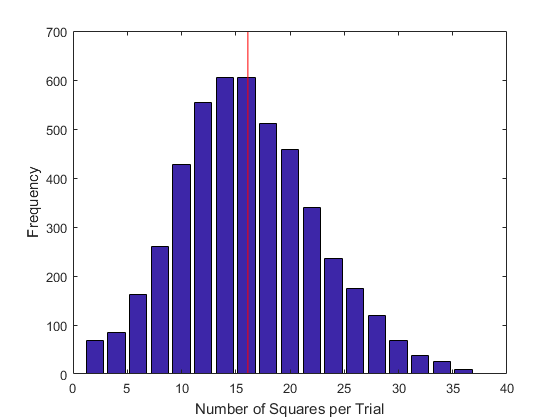
\includegraphics[width=0.8\textwidth]{exampleImage.png}
	\caption{Example caption}
	\label{fig:exampleImage}	
\end{figure} 

\begin{figure}[h!] % jou puts the images within the text. You will want the image to fit only half of the page, so the width is set to 0.5\text width. Change this to 1\test width to fill the whole page.
	\centering	
	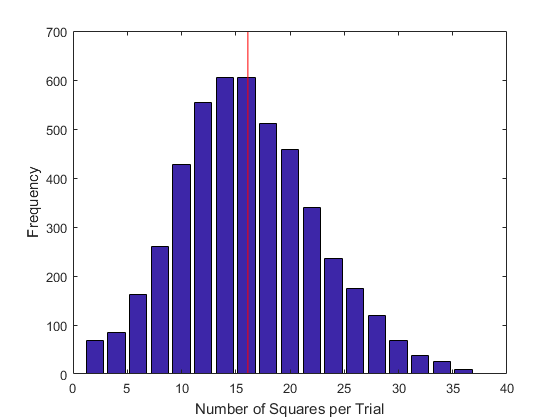
\includegraphics[width=0.5\textwidth]{exampleImage.png}
	\caption{Example caption}
	\label{fig:exampleImage}	
\end{figure} 

\section{Discussion}



% End of the manuscript

\section*{Acknowledgements}
Acknowledgements

\section*{Conflict of Interest Statement}

The authors declare that the research was conducted in the absence of any commercial or financial relationships that could be construed as a potential conflict of interest.

%\section*{Author Contributions}
% Un-comment this section to add author contributions


\section*{Data Accessibility Statement}
The raw data, pre-processed data, and analysis scripts can be found on the Open Science Framework: \url{url xx}

%\section*{Abbreviations}
% Un-comment this section to add abbreviations

\bibliography{bibliographyFileName}



\end{document}
